% Author: Dun-Ming Huang
% Email: dunmingbrandonhuang@berkeley.edu
% CSM16A Fall 2022

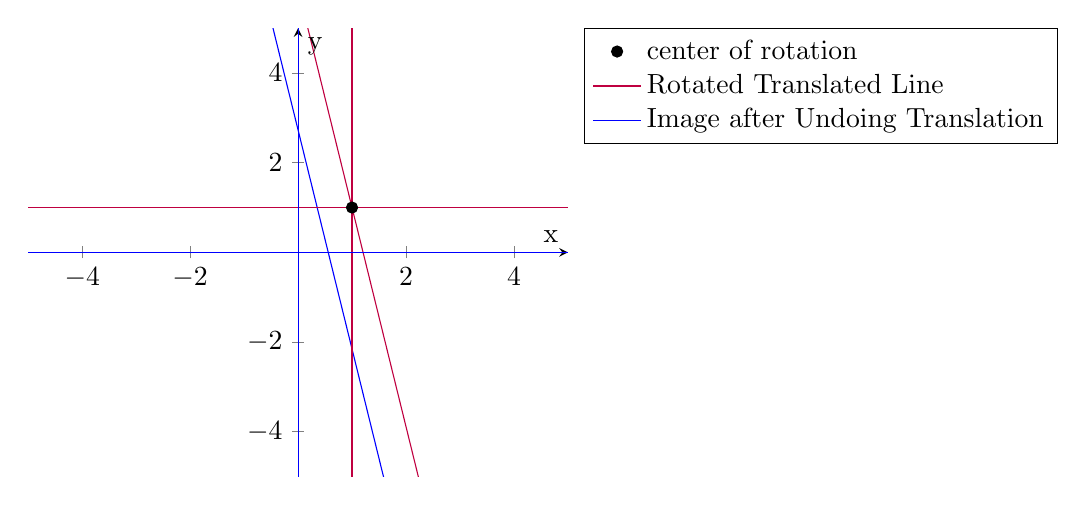
\begin{tikzpicture}
    \begin{axis}[
        axis lines = middle,
        xmin=-5, xmax=5,
        ymin=-5, ymax=5,
        xlabel = {x},
        ylabel = {y},
        legend pos=outer north east,
        legend cell align=left
    ]
        \addplot [only marks, color=black] table {
            1 1
        };
        \addlegendentry{center of rotation}
        \addplot [color=purple] {
           (6.196*x - 7.464) / -1.268
        };
        \addlegendentry{Rotated Translated Line}
        \addplot [color=blue] {
            (6.196*x - 3.464) / -1.268
        };
        \addlegendentry{Image after Undoing Translation}
        \addplot [color=purple] {
           1
        };
        \addplot [color=purple] coordinates {
            (1, -5) (1, 5)
        };
        \addplot [color=blue] {
           0
        };
        \addplot [color=blue] coordinates {
            (0, -5) (0, 5)
        };
        
    \end{axis}
\end{tikzpicture}